%

\chapter{Trójkąty}

% TODO: https://en.wikipedia.org/wiki/Triangle
% Sometimes an arbitrary edge is chosen to be the base, in which case the opposite vertex is called the apex; the shortest segment between the base and apex is the height. The area of a triangle equals one-half the product of height and base length.

%

% PRZECZYTANO: https://en.wikipedia.org/wiki/Pons_asinorum

\index{pons asinorum|(}

\section{Pons asinorum}

,,\emph{Pons asinorum}'', czyli most osłów, to tradycyjna nazwa twierdzenia (I.5), że kąty przy podstawie trójkąta równoramiennego są równe.
Ci, którzy nie są w stanie samodzielnie przeprowadzić jego dedukcyjnego dowodu opartego na własnościach trójkątów przystających, nie mogą przekroczyć mostu i studiować dalej geometrii.
Bardziej przyziemnie Coxeter \cite[s. 22-24]{coxeter_1967} zauważa, że rysunek wykonany przez Euklidesa przypomni most.
Wśród konsekwencji wymienia wyniki z~Elementów: (III.3), (III.20), (III.21), (III.22), (III.32), (VI.2), (VI.4), a potem (III.35), (III.36), (VI.19), co prowadzi do dowodu twierdzenia Pitagorasa, czyli (I.47).
\index{twierdzenie!Pitagorasa}%

\begin{figure}[H] \centering
\begin{comment}
\begin{tikzpicture}[scale=.5]
    \tkzDefPoint(90:-1){A}
    \tkzDefPoint(-55:5){C}
    \tkzDefPoint(235:5){B}
    \tkzDefPoint(-90:8){X}

    \tkzLabelPoint[above](A){$A$}
    \tkzLabelPoint[left](B){$B$}
    \tkzLabelPoint[right](C){$C$}
    \tkzInterLC(A,B)(A,X) \tkzGetPoints{XX}{D} % line and circle
    \tkzLabelPoint[left](D){$D$}
    \tkzDefLine[parallel=through D](B,C) \tkzGetPoint{XXX}
    \tkzInterLL(D,XXX)(A,C) \tkzGetPoint{E} % line and circle
    \tkzLabelPoint[right](E){$E$}
    
    \tkzMarkSegments[mark=|](A,B A,C)
    \tkzMarkSegments[mark=||](B,D C,E)
    \tkzDrawLines[add= 0 and 0, line width=0.2mm](B,E C,D)
    \tkzDrawLines[add= 0 and 0.5, line width=0.2mm](B,D C,E)
    \tkzDrawPolygon[line width=0.5mm](A,B,C)
    \tkzDrawPoints[size=4,color=black,fill=black!50](A,B,C,D,E)
\end{tikzpicture}
\end{comment}
    \caption{most osłów}
\end{figure}

Pierwsze dowody tego faktu podadzą jeszcze Euklides, komentujący jego prace Proklos, a także (dużo krócej\footnote{Pappus zauważa, że trójkąt $\triangle ABC$ przystaje do siebie $\triangle ACB$, więc stosowne kąty przy podstawie też są przystajace.}) Pappus z Aleksandrii.
\index[persons]{Proklos zwany Diadochem}%
\index[persons]{Pappus z Aleksandrii}%
Przyszłość przyniesie jeszcze jedno uzasadnienie, zaczynające się od wykreślenia dwusiecznej z kąta przy wierzchołku.
\index{dwusieczna}%
Euklides nie zrobi tego przede wszystkim ze względu na kolejność wykładanego materiału: dwusieczna pojawi się cztery tezy później, a nie można korzystać z wyników, których prawdziwości dopiero się pokaże.

O pons asinorum nie wspomina żaden szkolny podręcznik geometrii \texttt{:(}
Pojawia się u Bogdańskiej, Neugebauera \cite[s. 9]{neugebauer_2018}.

\index{pons asinorum|)}

\index{most osłów|see{pons asinorum}}

%
%

% PRZECZYTANO: https://en.wikipedia.org/wiki/Triangle_inequality

\section{Nierówność trójkąta}

\todofoot{https://www.deltami.edu.pl/2012/06/punkt-w-trojkacie/ zadanie 4 z odnośnikiem do tw. Ptolemeusza.}

Zajmiemy się teraz (I.20).

\begin{proposition}[nierówność trójkąta]
\index{nierówność!trójkąta}%
	Niech $ABC$ będzie trojkątem.
	Wtedy suma odcinków $AB$ i $BC$ jest dłuższa niż $AC$.
\end{proposition}

% TODO: https://www.deltami.edu.pl/2013/09/siatka-czworoscianu/ to samo w R3

\begin{proof}
	Wynika to ze wzoru Herona (fakt \ref{prp_heron}) i tego, że pole trójkąta jest nieujemne.
\end{proof}

\begin{corollary}
	Niech $a \ge b \ge c$ będą bokami trójkąta.
	Wtedy
	% \begin{equation}
	% 	1 < \frac{a + c}{b} < 3 
	% \end{equation}
	% oraz
	\begin{equation}
		1 \le \min \left(\frac ab, \frac bc\right) \le \phi = \frac {1 + \sqrt 5}{2}.
		% American Mathematical Monthly, pp. 49-50, 1954. 
	\end{equation}
\end{corollary}

Nierówność trójkąta nie jest wnioskiem z aksjomatów I1-I3, B1-B4, C1-C3, ponieważ nie zachodzi w następującym modelu (ukradniętym Hartshorne'owi \cite[s. 90]{hartshorne2000}):

\begin{example}
	Rozpatrujemy zbiór $\mathbb R^2$ jako płaszczyznę ze standardowymi punktami oraz prostymi, ale niestandardową metryką
	\begin{equation}
		d((x_1, y_1), (x_2, y_2)) = \begin{cases}
			\sqrt{(x_1-x_2)^2 + (y_1-y_2)^2} & \text{jeśli } x_1 = x_2 \vee y_1 = y_2, \\
			2 \sqrt{(x_1-x_2)^2 + (y_1-y_2)^2} & \text{w przeciwnym wypadku}
		\end{cases}.
	\end{equation}
	Wtedy nierówność trójkąta nie zachodzi.
\end{example}

Przytoczone niżej dwa zadania: Fagnano i Fermata będą prawie zawsze omawiane razem.

%

% https://en.wikipedia.org/wiki/Fagnano's_problem

\begin{problem}[zadanie Fagnano]
	Dany jest trójkąt ostrokątny $ABC$.
	Wpisać w niego trójkąt $DEF$ (czyli wybrać punkt $D$ na boku $BC$, $E$ na $AC$, $F$ na $AB$ tak, by tworzyły trójkąt) o możliwie najmniejszym obwodzie.
\index{zadanie!Fagnano}%
\end{problem}

Coxeter \cite[s. 36, 37]{coxeter_1967} pokaże tak jak Fejer, że rozwiązaniem zadania jest trójkąt spodkowy (którego wierzchołkami są spodki wysokości danego trójkąta; zwany brzydko ortycznym).
Zetel \cite[s. 97-100]{zetel_2020} przytoczy oprócz dowodu Fejera także dowód Izwolskiego, oparty na twierdzeniu: promienie okręgu opisanego na trójkącie, przechodzące przez wierzchołki trójkąta, są prostopadłe do odpowiednich boków trójkąta spodkowego.
Pompe \cite[s. 16-18]{pompe_2022} wykorzysta własności obrotów.
Audin \cite[s. 101]{audin_2003} podaje ten fakt w~formie ćwiczenia. % todo: fagnano czy gemrat?

Zadanie traci sens dla trójkątów nieostrokątnych: wtedy dwa z trzech wierzchołków trójkąta wpisanego o najmniejszym obwodzie pokrywają się z wierzchołkiem kąta rozwartego.

\begin{corollary}
	Wysokości trójkąta $ABC$ są dwusiecznymi kątów jego trójkąta spodkowego. % Pompe, Wokół obrotów, wniosek 2.3
\end{corollary}

Ten wniosek pojawia się u Zetela \cite[s. 89]{zetel_2020} i Pompego \cite[s. 19]{pompe_2022}.

\begin{proposition}
    Boki trójkąta spodkowego są antyrównoległe do boków trójkąta danego.
\end{proposition}

(Zetel \cite[s. 89]{zetel_2020}).

\begin{proposition}
	Niech wysokości trójkąta ABC przecinają sięw punkcie H.
	Każdy z czterech punktów A, B, C, H jest ortocentrum trójkąta, którego wierzchołkami są trzy pozostałe punkty.
\end{proposition}

(Zetel \cite[s. 95]{zetel_2020}).

%
%

\todofoot{https://www.deltami.edu.pl/2013/05/kacik-przestrzenny-17-punkt-fermata-torricellego/}
\todofoot{https://www.deltami.edu.pl/2018/01/zagadnienie-fermata-w-jednej-linijce/
}
\todofoot{https://www.deltami.edu.pl/2019/09/w-poszukiwaniu-trojkata-rownobocznego/ 14}
\todofoot{Zadanie Fermata -- Neugebauer, s. 117.}

\begin{problem}[zadanie Fermata]
	\label{punkt_fermata}
	Dany jest trójkąt ostrokątny $ABC$.
	Znaleźć punkt $P$ taki, by suma $|PA| + |PB| + |PC|$ była możliwie najmniejsza.
\index{zadanie!Fermata}%
\end{problem}

Powyższe zadanie rozwiąże Evangelista Torricelli (dlatego też punkt $P$ nazywa się czasem punktem Torricellego; robi tak Guzicki \cite[s. 224-228]{guzicki_2021}), który dostanie je w formie wyzwania od Fermata.
\index[persons]{Torricelli, Evangelista}%.
Rozwiązanie opublikuje student Torricelliego, Vincenzo Viviani, w 1659 roku.
\index[persons]{Viviani, Vincenzo}
% TODO: Johnson, R. A. Modern Geometry: An Elementary Treatise on the Geometry of the Triangle and the Circle. Boston, MA: Houghton Mifflin, pp. 221-222, 1929.
Coxeter \cite[s. 37]{coxeter_1967} przytoczy rozwiązanie Hofmanna\todofoot{J E Hoffman, Elementare Losung einer Mimimumsaufgabe 1929}
Patrz też Pompe \cite[s. 19-22]{pompe_2022}, Neugebauer \cite[s. 117]{neugebauer_2018}.
Audin \cite[s. 105]{audin_2003} podaje ten fakt w formie ćwiczenia.

Założenie ostrokątności można osłabić, wystarczy, żeby każdy kąt wewnętrzny trójkąta miał miarę mniejszą niż $2\pi/3$.

\begin{proposition}
    Dany jest trójkąt $ABC$, w którym żaden kąt nie ma miary większej niż $2\pi/3$.
    Wtedy wewnątrz istnieje dokładnie jeden punkt $P$ taki, że kąty $\angle APB$, $\angle BPC$, $\angle CPA$ są przystające (i miarę $2\pi/3$). 
\end{proposition}

Punkt $P$ jest punktem Fermata i można go łatwo skontruować.
Na zewnątrz boków trójkąta $ABC$ kreślimy trzy trójkąty równoboczne $ABD$, $BCE$, $CAF$, po czym prowadzimy proste $AE$, $BF$, $CD$.
Punkt $P$ leży na przecięciu wszystkich trzech, co wynika z twierdzenia Jacobiego:

\begin{proposition}
    Na bokach trójkąta $ABC$, po jego zewnętrznej stronie, zbudowano takie trójkąty $ABD$, $BCE$, $CAF$, że kąty: $\angle BAD = \angle CAF$, $\angle ABD = \angle CBE$, $\angle BCE = ACF$ są równe.
    Wówczas proste $AE$, $BF$, $CD$ przecinają się w jednym punkcie.
\end{proposition}

O twierdzeniu tym wspomni Pompe \cite[s. 21]{pompe_2022}, a następnie przejdzie do twierdzenia \ref{twierdzenie_ptolemeusza} (czyli Ptolemeusza).

%

%
%

\section{Punkty szczególne}

Z każdym trójkątem związane są pewne specjalne punkty, internetowa lista \emph{Encyclopedia of Triangle Centers} wymieni ich co najmniej 68 547.
My nie mamy aż tyle miejsca, więc ograniczymy się do najważniejszych.

$X(1)$ to środek okręgu wpisanego, 
$X(2)$ to środek ciężkości,
$X(3)$ to środek okręgu opisanego,
$X(4)$ to ortocentrum.
Te cztery punkty opisujemy poniżej.

$X(5)$ to środek okręgu dziewięciu punktów z faktu \ref{okrag_dziewieciu_punktow},
$X(6)$ to punkt Lemoine'a (Grebego) z faktu \ref{punkt_lemoine},
$X(7)$ to punkt Gergonne'a z~faktu \ref{punkt_gergonne},
$X(8)$ to punkt Nagela z faktu \ref{punkt_nagela}, 
$X(9)$ to mittenpunkt (punkt Lemoine'a trójkąta rozpiętego przez środki okręgów dopisanych; leży na prostych łączących środek ciężkości z punktem Gergonne'a, środek okręgu wpisanego z punktem Lemoine'a oraz ortocentrum ze środkiem Spiekera), % https://en.wikipedia.org/wiki/Mittenpunkt
$X(10)$ to środek okręgu Spiekera z faktu \ref{punkt_spiekera},
$X(11)$ to punkt Feuerbacha z twierdzenia \ref{punkt_feuerbacha},
$X(13)$ to punkt Fermata z zadania \ref{punkt_fermata},
$X(17)$, $X(18)$ to punkty Napoleona,
$X(39)$ to środek odcinka łączącego punkty Brocarda z definicji \ref{punkty_brocarda}.
Lista jest długa, a jej końca nie widać.

%

\subsection{Okrąg opisany i trzy symetralne}

\begin{proposition}
    \label{symetralne_przecinaja_sie}
    Trzy symetralne boków trójkąta przecinają się w jednym punkcie, środku okręgu opisanego na tym trójkącie.
\end{proposition}

Wynika to bezpośrednio z uwagi za definicją \ref{def_symetralna}: w trójkącie $\triangle ABC$, symetralna boku $AB$ (odpowiednio: $AC$) zawiera środki okręgów przechodzących przez punkty $A$ oraz $B$ (przez punkty $A$ oraz $C$), zatem trzecia symetralna musi przejść przez punkt wspólny dwóch pierwszych.

Hartshorne \cite[s. 16]{hartshorne2000} podaje to w formie ćwiczenia ze wskazówką, by spojrzeć na (IV.5).
Audin \cite[s. 61]{audin_2003} też, ale bez wskazówki.
Inne odsyłacze to Neugebauer \cite[s. 19]{neugebauer_2018}.

\begin{proposition}
	Środek okręgu opisanego na trójkącie leży wewnątrz tego trójkąta (odpowiednio: na jego brzegu, na zewnątrz trójkąta) wtedy i tylko wtedy, gdy trójkąt jest ostrokątny (odpowiednio: prostokątny, rozwartokątny).
\end{proposition}

Uogólnieniem faktu \ref{symetralne_przecinaja_sie} o współpękowości symetralnych boków trójkąta jest:

\begin{theorem}[Carnota]
\index{twierdzenie!Carnota}%
\label{guzicki_6_13}%
	Dany jest trójkąt $ABC$ i punkty $D, E, F$ leżące odpowiednio na prostych $BC, CA, AB$.
	Niech prosta $k$ (odpowiednio: $l$, $m$) przechodzi przez punkt $D$ ($E$, $F$) i będzie prostopadła do prostej $BC$ ($CA$, $AB$).
	Wtedy proste $k$, $l$, $m$ mają punkt wspólny wtedy i tylko wtedy, gdy
	\begin{equation}
		|AF|^2 + |BD|^2 + |CE|^2 = |AE|^2 + |BF|^2 + |CD|^2.
	\end{equation}
\end{theorem}
% TODO: https://en.wikipedia.org/wiki/Carnot%27s_theorem_(perpendiculars)

Guzicki \cite[s. 176]{guzicki_2021} wyprowadza je z twierdzenia Pitagorasa, co pozwala mu dojść do wniosku, że okręgi opisany i wpisany oraz ortocentrum istnieją.
\index{twierdzenie!Pitagorasa}

%
\subsection{Okrąg wpisany i trzy dwusieczne}

\begin{proposition}
    Trzy dwusieczne kątów trójkąta przecinają się w jednym punkcie, środku okręgu wpisanego w ten trójkąt.
\end{proposition}

Uzasadnienie jest kompletnie analogiczne do istnienia środku okręgu opisanego (tak zrobi Neugebauer \cite[s. 32]{neugebauer_2018}), ale można też podać fikuśny dowód dookoła: z twierdzenia o dwusiecznej i Cevy, jak Zetel \cite[s. 14]{zetel_2020}.
Hartshorne \cite[s. 16]{hartshorne2000} podaje to w formie ćwiczenia ze wskazówką, by spojrzeć na (IV.4), z czym totalnie się zgadzamy.

Po angielsku mamy krótkie określenia \emph{excenter, excircle, incenter, incircle}.

%

\subsection{Ortocentrum i trzy wysokości}

\begin{definition}[wysokość]
\index{wysokość trójkąta}%
    Niech $\triangle ABC$ będzie trójkątem, w którym przez punkt $C$ poprowadzono prostą prostopadłą do boku $AB$.
    Odcinek leżący na tej prostej, którego jeden koniec znajduje się w punkcie $C$, zaś drugi leży na boku $AB$, nazywamy wysokością opuszczoną z punktu $C$, drugi jego koniec to spodek wysokości.
\end{definition}

% TODO: Sometimes an arbitrary edge is chosen to be the base, in which case the opposite vertex is called the apex; the shortest segment between the base and apex is the height. The area of a triangle equals one-half the product of height and base length.

\begin{proposition}
\label{wysokosci_przecinaja_sie}%
	Trzy wysokości trójkąta (albo w przypadku trójkąta rozwartokątnego, przedłużenia wysokości) przecinają się w jednym punkcie zwanym ortocentrum (dawniej: środku ortycznym).
\index{ortocentrum}%
\end{proposition}

Dowodów we współczesnej literaturze nie brakuje: są u Pompego \cite[s. 38]{pompe_2022}, gdzie zmyślnie używa równoległoboków albo Guzickiego \cite[s. 218]{guzicki_2021}.
Warto też przeczytać tekst Hartshorne'a \cite[s. 54]{hartshorne2000} oraz Audina \cite[s. 61]{audin_2003}.
(Po angielsku mamy \emph{altitude}, \emph{foot of the altitude}, \emph{orthocenter}).

\begin{proposition}
    Dany jest trójkąt $ABC$ oraz jego ortocentrum $H$.
    Odbicia symetryczne punktu $H$ względem prostych zawierających boki trójkąta $ABC$ leżą na okręgu opisanym na tym trójkącie.
\end{proposition}

Dowód tego prostego stwierdzenia przedstawia Neugebauer \cite[s. 28]{neugebauer_2018}.

%
%

\subsection{Środek ciężkości i trzy środkowe}

\begin{definition}[środkowa]
\index{środkowa}%
    Dany jest pewien trójkąt.
    Odcinek łaczący którykolwiek z jego wierzchołków ze środkiem przeciwległego boku nazywamy środkową.
\end{definition}

Nie mylić z linią środkową!
Środkowe dzielą trójkąt na sześć mniejszych o równych polach.
% TODO: rysunek równych sześciu pól.

\begin{proposition}
    Niech $m_a, m_b, m_c$ oznacza długości trzech środkowych trójkąta, zaś $p$ połowę jego obwodu.
    Wtedy
    \begin{equation}
        \frac 32 p \le m_a + m_b + m_c \le 2p.
    \end{equation}
    % Posamentier, Alfred S., and Salkind, Charles T., Challenging Problems in Geometry, Dover, 1996: pp. 86–87.
\end{proposition}

Napisze o tym Coxeter \cite[s. 26]{coxeter_1967}.

\begin{proposition}
\label{srodkowe_przecinaja_sie}%
\index{środek ciężkości}%
    Trzy środkowe trójkąta przecinają się w jednym punkcie zwanym środkiem ciężkości i dzielą się w~stosunku $2$ do $1$, licząc od wierzchołków.
\end{proposition}
% % Coxeter, Introduction to Geometry, s. 10 <- przeczytaj to, nie tylko cytuj! + ćwiczenia: 3/4 <= 1

Środkowe to po angielsku \emph{medians}, przecinają się w \emph{centroid}.
Polska nazwa weźmie się z tego, że środek ciężkości fizycznego modelu trójkąta wykonanego z jednolitego materiału znajduje się właśnie tam.
\index{punkt!Spiekera}%
Angielska nazwa powstanie w 1814 roku z powodu niechęci do tego, co nie jest czysto geometryczne; niechęci, której nie będzie widać w innych europejskich językach.
(Środek ciężkości brzegu trójkąta nazywa się punktem Spiekera, patrz fakt \ref{punkt_spiekera}).

Hartshorne \cite[s. 52-54]{hartshorne2000} wnioskuje \ref{srodkowe_przecinaja_sie} z faktu \ref{hartshorne_52} (później zaś \cite[s. 119-120]{hartshorne2000} powtórzy dowód z~maszynerią geometrii analitycznej).
\index[persons]{Archimedes}%
Podobnie zrobią Guzicki \cite[s. 220]{guzicki_2021} albo Bogdańska, Neugebauer.
Zetel \cite[s. 14, 25]{zetel_2020} pokaże, że twierdzenie Cevy daje natychmiastowy dowód istnienia środka ciężkości.
\index{twierdzenie!Cevy}%
% TODO: Ich długość można obliczyć z https://en.wikipedia.org/wiki/Apollonius%27s_theorem => to jest z https://en.wikipedia.org/wiki/Median_(geometry)#Formulas_involving_the_medians'_lengths
Coxeter \cite[s. 26]{coxeter_1967} pokaże, jak otrzymać ten sam wynik z (VI.2) oraz (VI.4).

Historia faktów \ref{wysokosci_przecinaja_sie} oraz \ref{srodkowe_przecinaja_sie} ma wiele elementów wspólnych, więc omówimy je razem.
Żaden z nich nie pojawi się w Elementach Euklidesach i właściwie nie wiadomo, kto odkryje je pierwszy.
Uczeni arabscy stwierdzą, że był to Archimedes, choć nie ma ku temu niezbitych dowodów.
\index[persons]{Archimedes}%
Pappus będzie świadom istnienia ortocentrum, ale najstarsze znane uzasadnienie (w komentarzu al-Nasawiego) przyjdzie na świat dopiero w XI wieku.
\index[persons]{Pappus}%
\index[persons]{al-Nasawi, Ali ibn Ahmad}%

Fakt \ref{srodkowe_przecinaja_sie} ma trójwymiarową kontynuację:

\begin{proposition}
    Cztery odcinki łączące wierzchołki czworościanu ze środkami przeciwległych ścian przecinają się w~jednym punkcie, który dzieli je w stosunku $3$ do $1$.
\end{proposition}

Niektórzy stosują określenie ,,twierdzenie Commandino'', ponieważ Federico Commandino napisze w 1565 roku pracę \emph{De centro gravitatis solidorum} (O środkach ciężkości brył), chociaż może nie być pierwszym, który je odkrył.
\index{twierdzenie!Commandino}%
\index[persons]{Commandino, Federico}%
Podejrzewa się, że Francesco Maurolico pozna je wcześniej.
(Friederich Eduard Reusch znajdzie uogólnienie, które w zdegenerowanym przypadku prowadzi znowu do twierdzenia \ref{theorem_varignon} Varignona).
\index[persons]{Reusch, Friederich Eduard}%

%
%

\subsection{Prosta Simsona}

\todofoot{https://www.deltami.edu.pl/2011/09/o-prostej-simsona-raz-jeszcze/}
\todofoot{https://www.deltami.edu.pl/2015/10/prosta-simsona/}
\todofoot{https://www.deltami.edu.pl/2016/11/o-wlasnosciach-prostej-simsona/ + Steiner}
\todofoot{https://www.deltami.edu.pl/2018/09/o-ortocentrach-i-parabolach-a-zwlaszcza-o-twierdzeniu-odwrotnym-steinera/}

\begin{proposition}[twierdzenie Wallace'a]
	Dany jest trójkąt $ABC$ oraz punkt $P$.
	Niech $P_a$, $P_b$, $P_c$ oznacza rzuty punktu $P$ na proste $BC$, $AC$, $AB$.
	Wtedy następujące warunki są równoważne: punkt $P$ leży na okręgu opisanym na $\triangle ABC$; punkty $P_a$, $P_b$, $P_c$ są współliniowe.
\end{proposition}

Kiedy punkt $P$ leży na wspomnianym okręgu, prosta $P_aP_b$ nazywa się prostą Simsona; na cześć Roberta Simsona, szkockiego matematyka żyjącego w latach 1687-1768; chociaż pierwszą pracę na jej temat opublikuje Wallace w 1799 roku.
Być może właściwsze byłoby pisać ,,prosta Wallace'a-Simsona''.

Współliniowość spodków punktu $P$ na boki trójkąta jest twierdzeniem z dowodem u Zetela \cite[s. 55]{zetel_2020}, ćwiczeniem u Audina \cite[s. 104]{audin_2003} i Hartshorne'a \cite[s. 61]{hartshorne2000} i Neugebauera \cite[s. 25]{neugebauer_2018}.
% TODO: https://en.wikipedia.org/wiki/Simson_line
\todofoot{HARTSHORNE PRZECHODZI DO PUNKTU MIQUELA}

% PROSTA STEINERA? Audin ta sama strona
% http://users.math.uoc.gr/~pamfilos/eGallery/problems/SteinerLine.html

Z twierdzenia o prostej Wallace'a-Simsona wynika, jak u Zetela \cite[s. 57]{zetel_2020}:

\begin{proposition}[twierdzenie Salmona]
\index{twierdzenie!Salmona}% % https://ru.wikipedia.org/wiki/Теорема_Сальмона
	Dany jest okrąg oraz trzy jego różne cięciwy $PA$, $PB$, $PC$ takie, że przekrojem okręgów na średnicach $PA$, $PB$ (odpowiednio: $PB$, $PC$ i $PA$, $PC$) są punkty $P$, $M$ (odpowiednio: $P$, $K$ oraz $P$, $L$).
	Wtedy punkty $K$, $L$, $M$ są współliniowe.
\end{proposition}

%

%
%

\section{Twierdzenie Pitagorasa}

Najważniejszym twierdzeniem dotyczącym trójkątów prostokątnych jest twierdzenie Pitagorasa oraz twierdzenie do niego odwrotne.
Piszą o~nim Guzicki \cite[s. 160]{guzicki_2021}.

% PRZECZYTANO: https://en.wikipedia.org/wiki/Pythagorean_theorem

Do sformułowania twierdzenia Pitagorasa potrzebne jest pojęcie pola, którego z pewnych powodów nigdzie formalnie nie opisaliśmy.
Wystarczy nam wiedzieć, że dla każdej odpowiednio regularnej figury na płaszczyźnie $F$ istnieje liczba rzeczywista $S_F \ge 0$ (zwana polem) taka, że:
\begin{itemize}
    \item pole prostokąta o bokach długości $a$ oraz $b$ to $ab$;
    \item pole sumy (,,unii'') dwóch rozłącznych figur $F_1 \cup F_2$ jest sumą ich pól;
    \item pola przystających trójkątów są sobie równe.
\end{itemize}

(Można poczytać o tym u Neugebauera \cite[s. 37]{neugebauer_2018}).

\begin{theorem}[Pitagorasa]
\label{theorem_pythagorean}%
\index{twierdzenie!Pitagorasa}%
    Dany jest trójkąt prostokątny $\triangle ABC$, w~którym kąt przy wierzchołku $C$ jest prosty.
    Na jego bokach zbudowano trzy kwadraty.
    \begin{center}
\begin{comment}
        \begin{tikzpicture}[scale=.4]
        \tkzDefPoint(105:3){A}
        \tkzDefPoint(285:3){B}
        \tkzDefPoint(35:3){C}
        \tkzDefPoint(35:4.75){CC}
        \tkzMarkRightAngle[size=0.5](A,C,B)

        \tkzLabelPoint[above left](A){$A$}
        \tkzLabelPoint[below](B){$B$}
        \tkzLabelPoint[below left](CC){$C$}
        \tkzDefSquare(B,A)
        \tkzDrawPolygon[fill=black!50](B,A,tkzFirstPointResult, tkzSecondPointResult)
        \tkzDefSquare(C,B)
        \tkzDrawPolygon[fill=black!25](C,B,tkzFirstPointResult, tkzSecondPointResult)
        \tkzDefSquare(A,C)
        \tkzDrawPolygon[fill=black!25](A,C,tkzFirstPointResult, tkzSecondPointResult)
        \tkzDrawPolygon[line width=0.4mm](A,B,C)
    \end{tikzpicture}
\end{comment}
    \end{center}
    Suma pól jasnych kwadratów jest równa polu ciemnego kwadratu:
    \begin{equation}
        |AC|^2 + |BC|^2 = |AB|^2.
    \end{equation}
    Odwrotnie, jeśli $ABC$ jest trójkątem takim, że $|AC|^2 + |BC|^2 = |AB|^2$, to trójkąt ten jest prostokątny, zaś kąt przy wierzchołku $C$ jest prosty.
\end{theorem}

Powyższe twierdzenie przypiszemy kiedyś Pitagorasowi z~Samos, choć nie wiemy dokładnie, kto i~kiedy odkryje je jako pierwszy.
\index[persons]{Pitagoras z Samos}%
Będzie powszechnie stosowane w~okresie Starego Babilonu (XX-XVI wiek p.n.e.), a~więc na długo przed narodzinami Pitagorasa; pojawi się też w~indyjskich i~chińskich tekstach matematycznych.
Papirus Berlin 6619 spisany ok. 1800 roku p.n.e. na terenach państwa egipskiego zawrze zadanie, którego rozwiązaniem jest trójka $(6, 8, 10)$.
\index{papirus Berlin 6619}%
Jest jeszcze babilońska tabliczka Plimpton 322, także spisana ok. 1800 roku p.n.e., gdzie pojawia się trójka
\begin{equation}
    12709^2 + 13500^2 = 18541^2,
\end{equation}
co sugeruje, że jej autor znał pewną systematyczną metodę.
\index{tabliczka Plimpton 322}%

Być może twierdzenie Pitagorasa ma więcej znanych dowodów niż jakiekolwiek inne (poza prawem wzajemności reszt kwadratowych).
Będzie ich tak bardzo bez liku, że nie wiadomo, ile dokładnie.
Niektóre opierają się na rozcięciu pewnej układanki na fragmenty, przestawieniu ich i~zbudowaniu innego kształtu.
Inne korzystają z podobieństwa trójkątów.
Dowód Euklidesa urzekł nas tak bardzo swoją pomysłowością, że będzie jedynym, jaki przedstawimy w~całej książce!
\index{zasada!Cavalieriego}
Patrz też: Neugebauer \cite[s. 39-41]{neugebauer_2018}.

\begin{proof}
    Niech $\triangle ABC$ będzie trójkątem prostokątnym, z kątem prostym przy wierzchołku $C$.
    Na bokach $BC$, $AB$, $CA$ kreślimy kolejno kwadraty $BCDE$, $ABFG$, $ACHI$ (konstrukcja kwadratu Euklidesa korzysta z postulatu równoległości).

    \begin{center}
\begin{comment}
        \begin{tikzpicture}[scale=.4]
        \tkzDefPoint(105:3){A}
        \tkzDefPoint(285:3){B}
        \tkzDefPoint(35:3){C}
        \tkzDefPoint(35:4.75){CC}

        \tkzLabelPoint[above left](A){$A$}
        \tkzLabelPoint[below](B){$B$}
        \tkzLabelPoint[below left](CC){$C$}
        \tkzDefSquare(B,A)
        \tkzGetPoints{G}{F}
        \tkzLabelPoint[below](F){$F$}
        \tkzLabelPoint[above](G){$G$}
        \tkzDefPointsBy[projection=onto A--B](C){K}
        \tkzDefPointsBy[projection=onto G--F](C){L}

        \tkzDrawPolygon[line width=0.3mm, fill=blue!10](A,K,L,G)
        \tkzDrawPolygon[line width=0.3mm, fill=red!10](B,K,L,F)
        \tkzDrawPolygon[line width=0.3mm](A,B,F,G)
        \tkzLabelPoint[below left](K){$K$}
        \tkzLabelPoint[left](L){$L$}

        \tkzDefSquare(C,B)
        \tkzGetPoints{E}{D}
        \tkzDrawPolygon[line width=0.3mm,fill=red!40](C,B,E,D)
        \tkzLabelPoint[above](D){$D$}
        \tkzLabelPoint[below](E){$E$}
        \tkzDefSquare(A,C)
        \tkzGetPoints{H}{I}
        \tkzDrawPolygon[line width=0.3mm, fill=blue!40](A,C,H,I)
        \tkzLabelPoint[above right](H){$H$}
        \tkzLabelPoint[above right](I){$I$}
        \tkzDrawSegments[line width=0.2mm](C,G)
        \tkzDrawSegments[line width=0.2mm, dashed](C,K)
        \tkzDrawSegments[line width=0.2mm](I,B)
        % \tkzMarkRightAngle[size=0.5](A,C,B)
        \tkzDrawPolygon[line width=0.5mm](A,B,C)
    \end{tikzpicture}
\end{comment}
    \end{center}
    Z punktu $C$ opuszczamy wysokość na przeciwprostokątną\footnote{To jest jedno z dwóch wystąpień słowa przeciwprostokątna... :(} $AB$ i przedłużamy tak, by przecięła kwadrat $ABFG$ w punktach $K$ i $L$.
    Łączymy punkty $B$ i $I$ oraz $C$ i $G$.
    Otrzymane trójkąty $\triangle BAI$ oraz $\triangle GAC$ są przystające na mocy cechy bok-kąt-bok ($AB$, $\angle BAI$, $AI$ oraz $AG$, $\angle GAC$, $AC$).
    Niebieski prostokąt $AGLK$ (odpowiednio: kwadrat $ACHI$) ma dwukrotnie większe pole niż trójkąt $\triangle GAC$ (trójkąt $\triangle BAI$).
    (To jest zamaskowana zasada Cavalieriego!).
    \index{zasada Cavalieriego}%
    Zatem prostokąt $AGLK$ i~kwadrat $ACHI$ mają równe pola.
    
    Analogicznie pokazujemy, że czerwony prostokąt $BFLK$ i kwadrat $BCDE$ mają równe pola.
    Dodajemy dwie równości stronami i otrzymujemy, że suma pól kwadratów $ACIH$ oraz $BCDE$ jest równa polu kwadratu $ABFG$.
\end{proof}

Według legendy Hippazos z Metapontu odkryje, że przekątna kwadratu (albo, według innej legendy, pięciokąta) nie jest współmierna z~jego bokiem.
Niewymierność liczb $\sqrt{2}$ (albo $(1 + \sqrt 5) /2$) zrujnuje pogląd szkoły pitagorejskiej, że świat opiera się na liczbach (co dla ówczesnych znaczyć będzie: liczb naturalnych oraz ułamków z nich zbudowanych) i doprowadzi do utopienia Hippazosa.
\index[persons]{Hippazos z Metapontu}%
\index{utopienie}%
Ale jego śmierć nie cofnie rozłamu, jaki powstanie w szkole.
% TODO: https://www.deltami.edu.pl/2016/06/kwadraty/ Hippasus z Metapontu

(Być może w tym miejscu warto dowiedzieć się o cegle Eulera.)

\begin{corollary}
    Długość przekątnej prostokąta o bokach długości $a$ i $b$ wynosi $c = \sqrt{a^2 + b^2}$.
\end{corollary}

Kto umie rozwijać funkcje w szeregi potęgowe może wpaść na pomysł, by zapisać
\begin{equation}
    c = a + \frac{b^2}{2a} - \frac{b^4}{8a^3} + \frac{b^6}{16a^5} - \frac{5b^8}{127a^7} + \ldots,
\end{equation}
co po obcięciu do pierwszych dwóch wyrazów daje przybliżenie znane Babilończykom (\cite[s. 6]{eves1_1972}):
\begin{equation}
    c \approx a + \frac{b^2}{2a}.
\end{equation}

Metoda ta daje największy błąd względny, gdy $a = b$ i wynosi on $6.06601\ldots \%$.

\begin{problem} % Delta 2024/09
    Miasto jest otoczone okrągłym murem o nieznanej średnicy, z czterema bramami.
    Drzewo leży trzy nible na północ od północnej bramy.
    Jeśli idziemy dziewięć nibli na wschód od południowej bramy, drzewo staje się widoczne. 
    Znajdź średnicę miasta.
\end{problem}

Problem pochodzi z chińskiego tekstu \emph{Shu shu jiu zhang} (,,Traktat matematyczny w dziewięciu sekcjach'') z XIII wieku.
Jeżeli oznaczymy średnicę miasta przez $x$, odległość drzewa od miasta przez $b$, odległość do przejścia przez $a$, zaś kąt środek miasta -- punkt widoczności -- południowa brama przez $\alpha$, to dostaniemy równanie
\begin{equation}
    \tan 2 \alpha = 2 \tan \alpha + \frac ba,
\end{equation}
co po prostych przekształceniach i przyjęciu $y = \tan \alpha$ daje
$
    2ay^3 + by^2 - b = 0
$,
albo (pamiętając, że $y = x/2a$)
$
    x^3 + bx^2 - 4a^2 b = 0
$.
To równanie ma jedno rozwiązanie rzeczywiste, $x = 9$.

Względnie pierwsze liczby naturalne $a, b, c$ takie, że $a^2 + b^2 = c^2$ nazywamy (pierwotną) trójką pitagorejską.
\index{trójka pitagorejska}%
Każdą taką trójkę można otrzymać biorąc względnie pierwsze liczby $m, n$ różnej parzystości takie, że $m > n$ i kładąc $a = m^2 - n^2$, $b = 2 mn$, $c = m^2 + n^2$.
Najmniejszą taką trójką jest $(3, 4, 5)$; inna legenda (nie było w niej ani smoków, ani Hippazosa) głosi, że Egipcjanie używali tego trójkąta do wyznaczania kątów prostych u podstawy piramid.

\begin{proposition}
    Niech $\triangle ABC$ będzie trójkątem prostokątnym, z kątem prostym przy wierzchołku $C$:
    \begin{center}
\begin{comment}
    \begin{tikzpicture}[scale=.4]
        \tkzDefPoint(200:5){A}
        \tkzDefPoint(20:5){B}
        \tkzDefPoint(90:5){C}
        \tkzDefPointsBy[projection=onto A--B](C){D}
        \tkzLabelPoint[below left](200:5){A}
        \tkzLabelPoint[below right](22:5.3){B}
        \tkzLabelPoint[above](90:5.2){C}
        
        \tkzMarkRightAngle[size=0.8](A,C,B)
        \tkzDrawPolygons[line width=0.2mm](A,B,C)
        \tkzDrawSegment[dim={$\,\,p\,\,$,-8pt,transform shape,sloped}](A,D)
        \tkzDrawSegment[dim={$\,\,q\,\,$,-8pt,transform shape,sloped}](D,B)
        \tkzDrawSegment[dim={$\,\,b\,\,$,-8pt,transform shape,sloped}](C,A)
        \tkzDrawSegment[dim={$\,\,a\,\,$,-8pt,transform shape,sloped}](B,C)
        \tkzDrawPoints[size=3,color=black,fill=black!50](A,B,C)
        \tkzDrawSegment[dim={$\,\,h\,\,$,-0pt,transform shape,sloped}](C,D)
\end{tikzpicture}
\end{comment}
    \end{center}
    Mają wtedy miejsce następujące równości:
    \begin{equation}
        h = \frac{ab}{c}, \quad
        p = \frac{b^2}{c}, \quad
        q = \frac{a^2}{c}, \quad
        h^2 = pq.
    \end{equation}
\end{proposition}

Twierdzenie Pitagorasa znajduje zastosowanie także przy wyznaczaniu niektórych miejsc geometrycznych.

\begin{proposition}
    Dane są dwa różne punkty $A$ i $B$ na płaszczyźnie oraz liczba rzeczywista $c$ taka, że $2c > |AB|^2$.
    Miejscem geometrycznym punktów $P$ o własności $|AP|^2 + |BP|^2 = c$ jest okrąg o środku w środku odcinka $AB$ i średnicy $r = \sqrt{2c - |AB|^2}$.
\end{proposition}

\begin{proposition}
    Dane są dwa różne punkty $A$ i $B$ na płaszczyźnie oraz liczba rzeczywista $c$.
    Wtedy miejscem geometrycznym punktów $P$ o własności $|AP|^2 - |BP|^2 = c$ jest prosta prostopadła do prostej $AB$.
\end{proposition}

Patrz Guzicki \cite[s. 170-173]{guzicki_2021} (Guzicki wprowadza potem osie i środki potęgowe jak w~fakcie \ref{guzicki_6_11}, a następnie twierdzenie \ref{guzicki_6_13} (Carnota)).

Spirala Teodor(os)a z Cyreny składa się z trójkątów prostokątnych stykających się ze sobą wzdłuż boków.
\index{spirala Teodor(os)a}%
\index[persons]{Teodor(os) z Cyreny}%
Zaczynamy od trójkąta prostokątnego równoramiennego, o bokach długości $1$, $1$, $\sqrt{2}$, by następnie kreślić jednostkowy odcinek prostopadły do końca przeciwprostokątnej, łączymy go z~początkiem i powtarzamy (Teodoros zatrzyma się na trójkącie, którego najdłuższy bok to $\sqrt{17}$, ponieważ następny naszedłby na ten, od którego zaczynaliśmy).
\begin{figure}[H]\centering
\begin{comment}
    \begin{tikzpicture}[scale=.7]
        \tkzDefPoints{0.0000000000000000/0.0000000000000000/sqrt0,1.0000000000000000/0.0000000000000000/sqrt1,1.0000000000000002/1.0000000000000000/sqrt2,0.2928932188134524/1.7071067811865475/sqrt3,-0.6927053408400360/1.8762087599123103/sqrt4,-1.6308097207961914/1.5298560894922923/sqrt5,-2.3149821631755443/0.8005358106787454/sqrt6,-2.6417995393402450/-0.1445516998920071/sqrt7,-2.5871641322679750/-1.1430580705747615/sqrt8,-2.1830320757712630/-2.0577587215594090/sqrt9,-1.4971125019181266/-2.7854360801498297/sqrt10,-0.6162802729096475/-3.2588646221072777/sqrt11,0.3663043810988235/-3.4446801158290160/sqrt12,1.3606978771718410/-3.3389371493126440/sqrt13,2.2867524231255560/-2.9615474595774080/sqrt14,3.0782592751547995/-2.3503871670266260/sqrt15,3.6851266321570497/-1.5555840398277552/sqrt16,4.0740226421139890/-0.634302381788492/sqrt17}
        \tkzDrawPolygons[line width=0.2mm](sqrt0,sqrt1,sqrt2 sqrt0,sqrt2,sqrt3 sqrt0,sqrt3,sqrt4 sqrt0,sqrt4,sqrt5 sqrt0,sqrt5,sqrt6 sqrt0,sqrt6,sqrt7 sqrt0,sqrt7,sqrt8 sqrt0,sqrt8,sqrt9 sqrt0,sqrt9,sqrt10 sqrt0,sqrt10,sqrt11 sqrt0,sqrt11,sqrt12 sqrt0,sqrt12,sqrt13 sqrt0,sqrt13,sqrt14 sqrt0,sqrt14,sqrt15 sqrt0,sqrt15,sqrt16 sqrt0,sqrt16,sqrt17)
        \tkzMarkRightAngle[size=0.25](sqrt0,sqrt1,sqrt2)
        \tkzMarkRightAngle[size=0.25](sqrt0,sqrt2,sqrt3)
        \tkzMarkRightAngle[size=0.25](sqrt0,sqrt3,sqrt4)
        \tkzMarkRightAngle[size=0.25](sqrt0,sqrt4,sqrt5)
        \tkzMarkRightAngle[size=0.25](sqrt0,sqrt5,sqrt6)
        \tkzMarkRightAngle[size=0.25](sqrt0,sqrt6,sqrt7)
        \tkzMarkRightAngle[size=0.25](sqrt0,sqrt7,sqrt8)
        \tkzMarkRightAngle[size=0.25](sqrt0,sqrt8,sqrt9)
        \tkzMarkRightAngle[size=0.25](sqrt0,sqrt9,sqrt10)
        \tkzMarkRightAngle[size=0.25](sqrt0,sqrt10,sqrt11)
        \tkzMarkRightAngle[size=0.25](sqrt0,sqrt11,sqrt12)
        \tkzMarkRightAngle[size=0.25](sqrt0,sqrt12,sqrt13)
        \tkzMarkRightAngle[size=0.25](sqrt0,sqrt13,sqrt14)
        \tkzMarkRightAngle[size=0.25](sqrt0,sqrt14,sqrt15)
        \tkzMarkRightAngle[size=0.25](sqrt0,sqrt15,sqrt16)
        \tkzMarkRightAngle[size=0.25](sqrt0,sqrt16,sqrt17)
\end{tikzpicture}
\end{comment}
\caption{Spirala Teodor(os)a, zwany czasami ślimakiem pitagorejskim}
\end{figure}
\index{ślimak pitagorejski}%

%
%

\index{wzór!Herona|(}
\subsection{Pole trójkąta, wzór Herona}

\todofoot{delta 93-09}
\todofoot{https://www.deltami.edu.pl/2014/03/heron-uogolniony/}
\todofoot{https://www.deltami.edu.pl/2025/12/heron-heron-po-trzykroc-heron/}

W tej podsekcji znajdziemy różne wzory na pole trójkąta.

\begin{proposition}
    Pole trójkąta o podstawie długości $a$ oraz wysokości opuszczonej na tę podstawę długości $h$ wyraża się wzorem
    \begin{equation}
        S_\triangle = \frac 1 2 a h.
    \end{equation}
    Jeśli kąt naprzeciw podstawy ma miarę $\alpha$, a ramiona długości $b, c$, to zachodzi też
    \begin{equation}
        S_\triangle = \frac 1 2 bc \sin \alpha.
    \end{equation}
\end{proposition}

Pisze o tym Guzicki \cite[s. 255]{guzicki_2021}.

% TODO: https://www.cut-the-knot.org/Curriculum/Geometry/HeronsProblem.shtml#explanation

\begin{proposition}[wzór Herona, 60 r.n.e.?]
\label{prp_heron}%
    Pole trójkąta o bokach długości $a, b, c$ wyraża się wzorem
    \begin{equation}
        S = \sqrt{p(p-a)(p-b)(p-c)},
    \end{equation}
    gdzie $p = \frac 1 2 (a + b + c)$ oznacza połowę obwodu.
\end{proposition}

Wynik przypiszemy Heronowi z Aleksandrii, który poda dość skomplikowany dowód w~dziele \emph{,,Metrica''}.
\index[persons]{Heron z Aleksandrii}%
Coxeter \cite[s. 12]{coxeter_1991} przeczyta van der Waerdena \cite[s. 228, 277]{waerden_1961} i przez to stwierdzi, że wzór był już wcześniej znany Archimedesowi dwieście lat wcześniej; to samo pojawi się w polskim wydaniu \cite[s. 28]{coxeter_1967}.
% TODO: czemu jest cytowane angielskie i polskie wydanie?
\index[persons]{Archimedes}%
Pompe w $\Delta_{93}^9$ pokaże, jak dojść do dowodu Sidneya Kunga ,,bez rachowania''. % https://www.deltami.edu.pl/1993/09/jak-udowodnic-wzor-herona/
\index[persons]{Kung, Sidney}%
Guzicki \cite[s. 165-169]{guzicki_2021} wyprowadzi go z twierdzenia Pitagorasa i~wspomni, że prosty geometryczny dowód podał też Euler.
\index[persons]{Euler, Leonhard}%
\index{twierdzenie!Pitagorasa}
Wreszcie Bogdańska, Neugebauer \cite[s. 92]{neugebauer_2018} skorzystają z twierdzenia cosinusów.

Istnieje częściowe uogólnienie wzoru Herona dla czworokątów:

\begin{proposition}[wzór Brahmagupty]
    \label{brahmagupta_formula}%
    \index{czworokąt!cykliczny}%
    Pole czworokąta wypukłego, na którym można opisać okrąg, o bokach długości $a, b, c, d$ wyraża się wzorem
    \begin{equation}
        S = \sqrt{(p-a)(p-b)(p-c)(p-d)},
    \end{equation}
    gdzie $p$ oznacza połowę obwodu.
\end{proposition}
\index{wzór!Brahmagupty}%

Dowód polega na zastosowaniu wzoru Herona dwa razy do trójkątów podobnych lub ponownym skorzystaniu z dobrodziejstw trygonometrii.
Założenie o wypukłości i cykliczności można pominąć, jak odkryją równocześnie Carl Bretschneider i Karl von Staudt:
\index[persons]{Staudt@von Staudt, Karl}%
\index[persons]{Bretschneider, Carl}%

\begin{proposition}[wzór Bretschneidera, 1842]
    Pole czworokąta o bokach długości $a, b, c, d$ i sumie miar dwóch przeciwległych kątów wewnętrznych $2 \varphi$ wyraża się wzorem
    \begin{equation}
        S = \sqrt{(p-a)(p-b)(p-c)(p-d) - abcd \cos^2  \varphi},
    \end{equation}
    gdzie $p$ oznacza połowę obwodu.
\end{proposition}
\index{wzór!Bretschneidera}%

Inny, równie przydatny wzór znajdzie Julian Coolidge \cite{coolidge_1939}:
\index[persons]{Coolidge, Julian}%
pole czworokąta o bokach długości $a, b, c, d$ i przekątnych długości $e, f$ wyraża się wzorem
\begin{equation}
    S = \sqrt{(p-a)(p-b)(p-c)(p-d) - \frac 1 4 (ac + bd + pq)(ac + bd - pq)},
\end{equation}
gdzie $p$ oznacza raz jeszcze (i nie ostatni) połowę obwodu.

% TODO: https://en.wikipedia.org/wiki/History_of_geometry#Classical_Indian_geometry

\index{wzór!Herona|)}

%
%

\section{Okrąg dziewięciu punktów (Feuerbacha) i prosta Eulera}

\todofoot{https://www.deltami.edu.pl/2012/09/okrag-dziewieciu-punktow-i-pewne-dwa-fakty/}
\todofoot{https://www.deltami.edu.pl/2018/04/wysokosci-czworokata/ Monge}
\todofoot{https://www.deltami.edu.pl/2020/10/jego-wysokosci-czesc-2/}
\todofoot{https://www.deltami.edu.pl/2022/05/wspolliniowosc-i-katy/ i 20-10}

Prosta Eulera to pierwsza w szkolnej geometrii trójka punktów współliniowych.
Przyszła na świat w~1765 roku, w żurnalu \emph{Novi commentarii Academiae Petropolitanae}, w artykule \emph{Solutio facilis problematum quorundam geometricorum difficillimorum}, czyli jakbyśmy powiedzieli po polsku, ,,Łatwe rozwiązanie niektórych najtrudniejszych problemów geometrycznych''.

\begin{proposition}[prosta Eulera]
	\label{prosta_eulera}
	Środek okręgu opisanego na nierównobocznym trójkącie, środek ciężkości oraz ortocentrum leżą na jednej prostej, zwanej prostą Eulera.
	\index{prosta!Eulera}
\end{proposition}

Piszą o niej
Coxeter \cite[s. 32, 33]{coxeter_1967},
Hartshorne \cite[s. 54, 55]{hartshorne2000},
Guzicki \cite[s. 222]{guzicki_2021},
Bogdańska, Neugebauer \cite[s. 84]{neugebauer_2018},
Eves \cite[s. 109]{eves1_1972},
Audin \cite[s. 61]{audin_2003}.
W $\Delta_{84}^{4}$ podany będzie przepis, jak skonstruować trójkąt, w którym prosta Eulera ma zadane położenie względem podstawy.

\begin{proposition}
	Prosta Eulera jest prostopadła do jednego z boków trójkąta wtedy i tylko wtedy, gdy trójkąt jest równoramienny.
\end{proposition}

\begin{proposition}[okrąg dziewięciu punktów]
\label{okrag_dziewieciu_punktow}%
	W każdym trójkącie środki boków, spodki wysokości oraz środki odcinków łączących ortocentrum z wierzchołkami leżą na jednym okręgu.
	Jego środek pokrywa się ze środkiem odcinka łączącego środek okręgu opisanego z ortocentrum, zaś jego promień jest dwukrotnie krótszy od promienia okręgu opisanego.
	\index{okrąg!dziewięciu punktów}
\end{proposition}

% TODO: https://en.wikipedia.org/wiki/Nine-point_circle

Coxeter \cite[s. 34, 35, 88]{coxeter_1967},
Hartshorne \cite[s. 57, 60]{hartshorne2000},
Guzicki \cite[s. 223]{guzicki_2021},
Bogdańska, Neugebauer \cite[s. 85, 86]{neugebauer_2018},
Eves \cite[s. 109]{eves1_1972},
Audin \cite[s. 62]{audin_2003}.
Zetel \cite[s. 59, 85]{zetel_2020} (ze wzmianką o okręgu jedenastu punktów).

Temat badali Benjamin Bevan (który zasugerował środek oraz promień) i John Butterworth (który udowodnił podejrzenia Bevana) na początku XIX wieku.
\index[persons]{Bevan, Benjamin}%
\index[persons]{Butterworth, John}%
To, że środki boków i spodki wysokości leżą na wspólnym okręgu, zostało zauważone w 1821 roku przez Charles Brianchona i Jean-Victora Ponceleta.
\index[persons]{Brianchon, Charles}%
\index[persons]{Poncelet, Jean-Victor}%
Tego samego odkrycia dokonał rok później Karl Feuerbach; a krótko po nim Olry Terquem zauważył, że leży na nim dziewięć, a nie tylko sześć wspomnianych punktów.
\todofoot{The nine-point circle also passes through Kimberling centers Xi for i=11 (the Feuerbach point), 113, 114, 115 (center of the Kiepert hyperbola), 116, 117, 118, 119, 120, 121, 122, 123, 124, 125 (center of the Jerabek hyperbola), 126, 127, 128, 129, 130, 131, 132, 133, 134, 135, 136, 137, 138, 139, 1312, 1313, 1560, 1566, 2039, 2040, and 2679.}
\todofoot{Karl Wilhelm Feuerbach's Eigenschaften einiger merkwiirdigen Punkte des geradlinigen Dreiecks, along with many other interesting proofs relating to the nine point circle.}
\index[persons]{Feuerbach, Karl}%
\index[persons]{Terquem, Olry}%
Terquemowi (1842) zawdzięczamy nazwę ,,okrąg dziewięciu punktów''.
\todofoot{The circle is officially designated the "nine point circle" (le cercle des neuf points) by Terquem, one of the editors of the Nouvelles Annales. (see Volume I page 198).}
Zetel napisze, że Euler udowodnił je w 1765 roku w Petersburgu.

Feuerbach udowodnił też, że:

\begin{theorem}[Feuerbacha]
\label{punkt_feuerbacha}%
	Okrąg dziewięciu punktów jest styczny wewnętrznie do okręgu wpisanego (w punkcie Feuerbacha) i zewnętrznie do trzech okręgów dopisanych.
	\index{twierdzenie!Feuerbacha}%
\end{theorem}

Coxeter \cite[s. 99]{coxeter_1967}, Audin \cite[s. 110]{audin_2003} podają ten fakt w formie ćwiczenia.
Eves \cite[s. 133]{eves1_1972} podaje pełne uzasadnienie.
Zetel \cite[s. 70]{zetel_2020} bardzo prosto dowodzi, że punkty styczności można znaleźć bez konstruowania pięciu okręgów.

\begin{proposition}
	\label{orthic_triangle}
	Niech $ABC$ będzie trójkątem ostrokątnym, zaś $K$, $L$ oraz $M$ spodkami jego wysokości.
	Wtedy wysokości trójkąta $ABC$ są dwusiecznymi kątów trójkąta $KLM$.
\end{proposition}

Hartshorne \cite[s. 58]{hartshorne2000}.

\begin{theorem}[Hamiltona]
	Dany jest trójkąt $ABC$ oraz jego ortocentrum $H$.
	Wtedy okręgi dziewięciu punktów trójkątów $ABC$ oraz $ABH$ są identyczne: mają ten sam środek i promień.
\end{theorem}

O twierdzeniu Hamiltona pisze Zetel \cite[s. 65]{zetel_2020}; rzekomo pierwszy dowód poda Hamilton w 1861 roku.

\begin{corollary}
	Okręgi opisane na trójkątach $ABC$, $ABH$, $BCH$, $ACH$ mają równe promienie.
\end{corollary}

%

\section{Nierówności trójkątne}

\todofoot{Coxeter, s. 12}
\todofoot{https://www.deltami.edu.pl/2016/06/boki-trojkata/}

\begin{proposition}[nierówność izoperymetryczna]
	Dany jest trójkąt o połowie obwodu $p$ oraz polu $S$.
	Wtedy 
	\begin{equation}
		S \le \frac{p^2}{3 \sqrt 3},
	\end{equation}
	zatem wśród trójkątów o ustalonym obwodzie największe pole ma trójkąt równoboczny.
	\index{nierówność!izoperymetryczna}
	% TODO: https://www.deltami.edu.pl/2011/04/symetryzacja-steinera/
\end{proposition}

https://www.deltami.edu.pl/2023/01/nierownosc-izoperymetryczna/

Guzicki \cite[s. 169, 170]{guzicki_2021} wyprowadza nierówność izoperymetryczną ze wzoru Herona oraz nierówności między średnią arytmetyczną i~geometryczną.
\index{wzór!Herona}%
Odpowiednik tego w trzech wymiarach znany będzie jako hipoteza (Zdzisława Aleksandra) Melzaka: podana około roku 1965, będzie musiała długo czekać na swoje rozwiązanie.
\index[persons]{Melzak, Zdzisław Aleksander}%
% trójwymiarowy odpowiednik to hipoteza: https://math.stackexchange.com/questions/4044670/what-is-the-largest-volume-of-a-polyhedron-whose-skeleton-has-total-length-1-is
\begin{proposition}[nierówność Eulera]
\index{nierówność!Eulera}%
	Niech $R, r, d$ oznaczają kolejno promienie okręgu opisanego i wpisanego w~trójkąt oraz odległość między środkami tych okręgów.
	Wtedy
	\begin{equation}
	\frac{1}{R-d} + \frac{1}{R+d} = \frac 1 r,
	\end{equation}
	lub równoważnie $d^2 = R \cdot (R - 2r)$.
	Wynika stąd, że $R \ge 2r$.
\end{proposition}

https://www.deltami.edu.pl/2019/03/twierdzenie-o-trojzebie/

Leonhard Euler opublikuje ten wynik w 1765 roku, chociaż wcześniej zrobi to William Chapple, w pracy \emph{,,An essay on the properties of triangles inscribed in and circumscribed about two given circles''} z 1746 roku, na dole strony 123.
% Leversha, Gerry; Smith, G. C. (November 2007), "Euler and triangle geometry", The Mathematical Gazette, 91 (522): 436–452, doi:10.1017/S0025557200182087, JSTOR 40378417, S2CID 125341434
% TODO: https://en.wikipedia.org/wiki/Euler%27s_theorem_in_geometry a stornger version... [6]
Wspomni go Zetel \cite[s. 75]{zetel_2020}

Trójwymiarowym odpowiednikiem jest:

\begin{proposition}[nierówność Grace'a-Danielssona]
\index{nierówność!Grace'a-Danielssona}%
	Dla każdej pary sfer o promieniach $r, R$ takich, że $r < R$ istnieje czworościan zawarty w dużej sferze i zawierający małą sferę wtedy i tylko wtedy, gdy
	\begin{equation}d^2 \le (R+r)(R - 3r).\end{equation}
\end{proposition}
% TODO: Grace, J.H. (1918), Proc. London Math. (ed.), Tetrahedra in relation to spheres and quadrics, vol. Soc.17, pp. 259–271
% Danielsson, G. (1952), Johan Grundt Tanums Forlag (ed.), Proof of the inequality d2≤(R+r)(R−3r) for the distance between the centres of the circumscribed and inscribed spheres of a tetrahedron, pp. 101–105
%

\begin{proposition}[nierówność Mitrinovica]
	Niech...
	\index{nierówność!Mitrinovica}
\end{proposition}

%
%

\begin{proposition}[nierówność Leibniza]
	Niech...
	\index{nierówność!Leibniza}
\end{proposition}

%
%

\subsection{Nierówność Weitzenböcka i jej uogólnienia}

% https://en.wikipedia.org/wiki/Weitzenböck's_inequality

Roland Weitzenböck \cite{weitzenbock_1919} udowodni w 1919 roku:
\index[persons]{Weitzenböck, Roland}%

\begin{proposition}[nierówność Weitzenböcka]
	W trójkącie o bokach długości $a, b, c$ oraz polu powierzchni $S$ zachodzi nierówność
    \begin{equation}
        a^2 + b^2 + c^2 \ge 4 \sqrt{3} S,
    \end{equation}
    z równością wtedy i tylko wtedy, gdy trójkąt jest równoboczny: $a = b = c$.
	\index{nierówność!Weitzenböcka}%
\end{proposition}

% https://en.wikipedia.org/wiki/Weitzenböck%27s_inequality#Further_proofs
Dowód wykorzystuje punkt Fermata, wzór Herona, nierówność między średnią arytmetyczną i~geometryczną, własności funkcji cotangens albo nierówność
\begin{equation}
    (a^2 - b^2)^2 + (b^2 - c^2)^2 + (c^2 - a^2)^2 \ge 0.
\end{equation}
\index{punkt Fermata}%
\index{wzór Herona}%
% https://www.ime.usp.br/~toscano/disc/2022/GreenbergGeometry.pdf ps. 34

Są dwa uogólnienia: nierówność Hadwigera-Finslera oraz nierówność (Neuberga-)Pedoego.

\begin{proposition}[nierówność Hadwigera-Finslera]
    W trójkącie o bokach długości $a, b, c$ oraz polu powierzchni $S$ zachodzi nierówność
    \begin{equation}
        a^2 + b^2 + c^2 \ge (a-b)^2 + (b-c)^2 + (a-c)^2 + 4 \sqrt{3} S,
    \end{equation}
\end{proposition}

\begin{proof}
    Z twierdzenia cosinusów mamy $a^2 = b^2 + c^2 - 2bc \cos \alpha$.
    Ponieważ $S = \frac 1 2 b c \sin \alpha$, poprzednią równość możemy przepisać do 
    \begin{align}
        a^2 & = (b-c)^2 + 4S \cdot \frac{1 - \cos \alpha}{\sin \alpha} \\
        & = (b-c)^2 + 4S \cdot \frac{2 \sin^2 (\alpha / 2)}{2 \sin (\alpha / 2) \cos (\alpha / 2)} \\
        & = (b-c)^2 + 4S \cdot \tan \frac \alpha 2.
    \end{align}
    Po powtórzeniu tego dla pozostałych boków i dodaniu do siebie dostaniemy
    \begin{equation}
        a^2 + b^2 + c^2 = (a-b)^2 + (b-c)^2 + (c-a)^2 + 4S \left(\tan \frac \alpha 2 + \tan \frac \beta 2 + \tan \frac \gamma 2\right).
    \end{equation}
    Ale połówki kątów trójkąta nie przekraczają $\pi/2$, zaś funkcja $\tan$ jest wypukła, więc nawias można ograniczyć z dołu:
    \begin{equation}
        \tan \frac \alpha 2 + \tan \frac \beta 2 + \tan \frac \gamma 2 \ge 3 \tan \frac{\alpha + \beta + \gamma}{6} = 3\tan \frac \pi 6 = \sqrt 3,
    \end{equation}
    co kończy dowód.
\end{proof}

Paul Finsler oraz Hugo Hadwiger \cite{finsler_1937} udowodnią to twierdzenie w 1937 roku.
\index[persons]{Finsler, Paul}%
\index[persons]{Hadwiger, Hugo}%

\begin{proposition}[nierówność Neuberga-Pedoego]
    W dwóch trójkątach o bokach $a, b, c$ oraz polu powierzchni $S$ i bokach $a_*, b_*, c_*$ oraz polu powierzchni $S_*$ zachodzi nierówność
    \begin{equation}
        a^2_*(b^2 + c^2 - a^2) + 
        b^2_*(a^2 + c^2 - b^2) + 
        c^2_*(a^2 + b^2 - c^2) \ge 16 SS_*
    \end{equation}
    z równością wtedy i tylko wtedy, gdy trójkąty są podobne: $a/a_* = b/b_* = c/c_*$.
\end{proposition}

(Aby dostać nierówność Weitzenböcka, wystarczy wziąć $a = b = c = 1$).
Daniel Pedoe \cite{pedoe_1941} odkryje nierówność w 1941, a później dowie się, że była znana luksemburskiemu geometrze Józefowi Neubergowi.
\index[persons]{Pedoe, Daniel}%
\index[persons]{Neuberg, Joseph}%
Ten jednak nie pokaże, że z równości dwóch strony wynika podobieństwo trójkątów.
Jeden z dowodów wykorzystuje wzór Herona oraz nierówność Cauchy'ego-Schwarza.

%
%

\subsection{Nierówność Ono}

% https://en.wikipedia.org/wiki/Ono%27s_inequality

W 1914 roku Toda Ono wysnuje hipotezę (nieprawdziwą w ogólności, ale prawdziwą dla wszystkich trójkątów ostrokątnych): % 小野藤太
\index[persons]{Ono, Toda}%

\begin{proposition}[nierówność Ono]
    W trójkącie ostrokątnym o bokach długości $a, b, c$ oraz polu powierzchni $S$ zachodzi nierówność
    \begin{equation}
        \frac{27}{4096} \cdot (b^2 + c^2 - a^2)^2 (c^2 + a^2 - b^2)^2 (a^2 + b^2 - c^2)^2 \le S^6.
    \end{equation}
\end{proposition}

Dowód znajdzie F. Balitrand w 1916 roku.
\index[persons]{Balitrand, F?}%
% Ono, T. (1914). "Problem 4417". Interméd. Math. 21: 146.
% https://zbmath.org/?format=complete&q=an:46.0859.06
Nierówność nie zachodzi dla trójkąta o bokach długości $a = 2$, $b = 3$, $c = 4$, wtedy $S^2 = 135/16$.

%
%

\index{nierówność!Erdősa-Mordella|(}

\subsection{Nierówność Erdősa-Mordella i jej uogólnienie}

\begin{theorem}[nierówność Erdősa-Mordella]
    Niech $P$ będzie punktem wewnątrz trójkąta $\triangle ABC$, zaś $A_p, B_p, C_p$ spodkami punktu $P$ na boki trójkąta jak na rysunku \ref{erdos_mordell_barrowa}.
    Wtedy
    \begin{equation}
        |PA| + |PB| + |PC| \ge 2 (|PA_p| + |PB_p| + |PC_p|).
    \end{equation}
\end{theorem}

\begin{figure}[H] \centering
\begin{minipage}[b]{.45\linewidth}
\begin{center}
    \begin{comment}
    \begin{tikzpicture}[scale=.4]
    \tkzDefPoint(0, 0){A}
    \tkzDefPoint(10, 2){B}
    \tkzDefPoint(6, 7){C}
    \tkzDefPoint(5, 3){P}
    \tkzLabelPoint[below left](A){$A$}
    \tkzLabelPoint[below right](B){$B$}
    \tkzLabelPoint[above](C){$C$}
    \tkzLabelPoint[below left](P){$P$}
    \tkzDefPointsBy[projection=onto A--B](P){Pc}
    \tkzDefPointsBy[projection=onto B--C](P){Pa}
    \tkzDefPointsBy[projection=onto C--A](P){Pb}
    \tkzLabelPoint[above right](Pa){$A_p$}
    \tkzLabelPoint[above left](Pb){$B_p$}
    \tkzLabelPoint[below](Pc){$C_p$}

    \tkzDrawSegments[line width=0.2mm,dashed](P,Pa P,Pb P,Pc)
    \tkzDrawPolygon[line width=0.3mm](A,B,C)
    \tkzMarkRightAngles[size=0.5](P,Pa,C P,Pb,A P,Pc,B)
    \tkzDrawPoints[size=3,color=black,fill=black!50](A,B,C,P,Pc,Pb,Pa)
\end{tikzpicture}
\end{comment}
    \end{center}
    \subcaption{nierówność Erdősa-Mordella}
    \label{erdos_mordell_barrowa}
\end{minipage}
%
\begin{minipage}[b]{.45\linewidth}
\begin{center}\begin{comment}
    \begin{tikzpicture}[scale=.4]
    \tkzDefPoint(0, 0){A}
    \tkzDefPoint(10, 2){B}
    \tkzDefPoint(6, 7){C}
    \tkzDefPoint(5, 3){P}

    \tkzDefLine[bisector](A,P,B) \tkzGetPoint{prePc}
    \tkzInterLL(P,prePc)(A,B) \tkzGetPoint{Pc}
    \tkzDefLine[bisector](B,P,C) \tkzGetPoint{prePa}
    \tkzInterLL(P,prePa)(B,C) \tkzGetPoint{Pa}
    \tkzDefLine[bisector](C,P,A) \tkzGetPoint{prePb}
    \tkzInterLL(P,prePb)(C,A) \tkzGetPoint{Pb}

    \tkzLabelPoint[below left](A){$A$}
    \tkzLabelPoint[below right](B){$B$}
    \tkzLabelPoint[above](C){$C$}
    %\tkzLabelPoint[below left](P){$P$}
    \tkzLabelPoint[above right](Pa){$A_p$}
    \tkzLabelPoint[above left](Pb){$B_p$}
    \tkzLabelPoint[below](Pc){$C_p$}

    \tkzMarkAngle[arc=lll,size=1.2,mark=|||](A,P,Pc)
    \tkzMarkAngle[arc=lll,size=1.2,mark=|||](Pc,P,B)
    \tkzMarkAngle[arc=ll,size=1.2,mark=||](B,P,Pa)
    \tkzMarkAngle[arc=ll,size=1.2,mark=||](Pa,P,C)
    \tkzMarkAngle[arc=l,size=1.2,mark=|](C,P,Pb)
    \tkzMarkAngle[arc=l,size=1.2,mark=|](Pb,P,A)

    \tkzDrawSegments[line width=0.2mm](P,A P,B P,C)
    \tkzDrawSegments[line width=0.2mm,dashed](P,Pa P,Pb P,Pc)
    \tkzDrawPolygon[line width=0.3mm](A,B,C)
    \tkzDrawPoints[size=3,color=black,fill=black!50](A,B,C,P,Pc,Pb,Pa)
\end{tikzpicture}
\end{comment}
    \end{center}
    \subcaption{nierówność Barrowa}
    \label{erdos_mordell_barrowb}
\end{minipage}
\caption{}
\end{figure}

\label{subsection_erdos_mordell}
Nierówność pojawi się w wakacyjnym wydaniu American Mathematical Monthly z 1935 roku jako problem 3740 od Erdősa.
\index[persons]{Erdős, Paul}%
Na dowód przyjdzie poczekać.
Pierwszy podadzą Louis Mordell i~David Barrow \cite{mordell_barrow_1937} w 1937 roku.
\index[persons]{Mordell, Louis Joel}%
\index[persons]{Barrow, David}%
Po dwudziestoletniej przerwie pojawi się prostszy dowód Kazarinowa \cite{kazarinoff_1957};
\index[persons]{Kazarinoff, Donat}% Donat Konstantinovich Kazarinoff
Leon Bankoff \cite{bankoff_1958} uzasadni nierówność wykorzystując jedynie podobieństwo trójkątów oraz fakt, że $t + 1/t \ge 2$ dla $t \ge 0$; cały dowód zmieści się na połowie strony w $\Delta_{90}^8$.
\index[persons]{Bankoff, Leon}%
Ostatni współczesny dowód pochodzi od Claudi Alsiny i Rogera Nelsena \cite{alsina_2007}.
\index[persons]{Alsina, Claudi}%
\index[persons]{Nelsen, Roger}%

% https://en.wikipedia.org/wiki/Erdős-Mordell_inequality
Coxeter \cite[s. 25]{coxeter_1967} przetworzy je po latach w ćwiczenie dla Czytelnika;
podobnie postąpi Audin \cite[s. 102]{audin_2003}, nie szczędząc przy tym wskazówek.
W geometrii absolutnej nierówność Erdősa-Mordella jest równoważna temu, że suma kątów trójkąta nie przekracza $\pi$ (patrz Pambuccian \cite{pambuccian_2008}).
\index[persons]{Pambuccian, Victor}%

Wzmocnieniem nierówności Erdősa-Mordella będzie nierówność Barrowa:
\index{nierówność!Barrowa}

% TODO: https://en.wikipedia.org/wiki/Barrow%27s_inequality

\begin{theorem}[nierówność Barrowa]
    Niech $P$ będzie punktem wewnątrz trójkąta $\triangle ABC$, zaś $A_p$, $B_p$, $C_p$ punktami przecięć dwusiecznych trzech kątów wyznaczanych przez $P$ i pary wierzchołków trójkąta; tak jak na rysunku \ref{erdos_mordell_barrowb}.
    Wtedy
    \begin{equation}
        |PA| + |PB| + |PC| \ge 2 (|PA_p| + |PB_p| + |PC_p|).
    \end{equation}
\end{theorem}

Dowód Barrowa i Mordella \cite{mordell_barrow_1937} zostanie opublikowany w 1937 roku, ale nazwa ,,nierówność Barrowa'' przyjmie się nieco później, na pewno w 1961 roku Alexander Oppenheim będzie już jej używać.
\index[persons]{Oppenheim, Alexander}%
% Oppenheim, A. (1961), "New inequalities for a triangle and an internal point", Annali di Matematica Pura ed Applicata, 53: 157–163, doi:10.1007/BF02417793, MR 0124774
Mordell \cite{mordell_1962} wróci do nierówności po latach i poda prostszy dowód.
\index[persons]{Mordell, Louis Joel}%

\index{nierówność!Erdősa-Mordella|)}

% % barrow tu jest

\subsection{Nierówności trygonometryczne}
%

\index{nierówność!Mikołaja z Kuzy|(}

\begin{proposition}[nierówność Mikołaja z Kuzy]
\begin{equation}
	\label{nierownosc_mikolaja_z_kuzy}
	\frac{\sin x}{x} < \frac{2 + \cos x}{3}.
\end{equation}
\end{proposition}

Mikołaj z Kuzy (znany też jako Kuzańczyk) w wielu pismach zajmie się problemem kwadratury koła i obliczania obwodu koła.
\index[persons]{Mikołaj z Kuzy}%
Jego przybliżenie $\pi \approx 6\sqrt{48/7}/5 = 3.1423...$ (z \emph{De Geometricis Transmutationibus} z 1445 roku) będzie zgodne z~oszacowaniem $223/71 < \pi < 22/7$ pochodzącym jeszcze od Archimedesa.
Niestety, późniejsze pomysły będą mniej trafione; 
Regiomontanus omówi po kolei wszystkie konstrukcje Mikołaja i~przejdzie do liczb (,,\emph{nunc ad numeros descendendum}'').
Policzy na przykład, że Mikołaj w \emph{Quadratura Circuli} z 1450 roku sugeruje $\pi = 3.154\ldots > 22/7$. 

\index{nierówność!Mikołaja z Kuzy|)}

https://www.deltami.edu.pl/2020/03/o-nierownosci-miedzy-srednia-arytmetyczna-sinusa-i-tangensa-kata-ostrego-a-jego-miara/

%
%

\index{nierówność!Snelliusa-Huygensa}%
\begin{proposition}[nierówność Snelliusa-Huygensa]
	\begin{equation}
		2 \sin x + \tan x > 3x.
		\label{nierownosc_snelliusa}
	\end{equation}
\end{proposition}

Willebrod Snellius poda zawiły dowód w książce Cyclometicus (1631); schludniejsze uzasadnienie znajdzie Christian Huygens.
\index[persons]{Snellius, Willebrod}%
\index[persons]{Huygens, Christian}%
W \emph{,,De circuli magnitudine inventa''} użyje nierówności \ref{nierownosc_mikolaja_z_kuzy} oraz \ref{nierownosc_snelliusa} do oszacowania wartości $\pi$.

%

% https://www.awesomemath.org/wp-pdf-files/math-reflections/mr-2025-04/mr_4_2025_trigonometric_inequalities_v2.pdf


%

\section{Okrąg Spiekera}
%

\begin{proposition}[punkt i okrąg Spiekera]
\label{punkt_spiekera}%
    Niech $\triangle ABC$ będzie trójkątem.
    Środek okręgu wpisanego w trójkąt, którego wierzchołkami są środki boków trójkąta $ABC$, nazywamy jego punktem Spiekera.    
\end{proposition}

O punkcie Spiekera pisze też Zetel \cite[s. 22]{zetel_2020}, chociaż nie nazywa go tak, być może dlatego, że Theodor Spieker będzie dziewiętnastowiecznym geometrą z Niemiec (Poczdamu)?
\index[persons]{Spieker, Theodor}

https://www.deltami.edu.pl/2011/11/srodek-ciezkosci/

%
%

\section{Twierdzenie Talesa}

\todofoot{Guzicki-3}

\begin{theorem}[Talesa]
\index{twierdzenie!Talesa}%
    Jeśli ramiona kąta płaskiego przetnie się 2 równoległymi prostymi:
    \begin{center}
\begin{comment}
        \begin{tikzpicture}
            \tkzDefPoint(0, 0.5){O}
            \tkzDefPoint(1.5, 0){A}
            \tkzDefPoint(2, 1){Ap}
            \tkzDefPointBy[homothety=center O ratio 1.618](A) \tkzGetPoint{B}
            \tkzDefLine[parallel=through B](A,Ap) \tkzGetPoint{Bp}
            \tkzInterLL(O,Ap)(B,Bp) \tkzGetPoint{Bpp}
            \tkzDrawPoints[fill=gray,opacity=.9](O,A,B,Ap,Bpp)
            \tkzLabelPoint[above](O){$O$}
            \tkzLabelPoint[below](A){$A$}
            \tkzLabelPoint[below](B){$A'$}
            \tkzLabelPoint[above left](Bpp){$B'$}
            \tkzLabelPoint[above left](Ap){$B$}
            \tkzDrawLine[thick](O,B)
            \tkzDrawLine[thick](O,Bpp)
            \tkzDrawLine[color=blue, thick](A,Ap)
            \tkzDrawLine[color=blue, thick](B,Bpp)
        \end{tikzpicture}
\end{comment}
        \end{center}
    to długości odcinków wyznaczonych przez te proste na jednym z ramion kąta są proporcjonalne do długości odpowiednich odcinków na drugim ramieniu kąta, a zatem
    \begin{equation}
        \label{thales_ratio}
        \frac{|OA|}{|OA'|} = \frac{|OB|}{|OB'|} = \frac{|AB|}{|A'B'|}.
    \end{equation}
\end{theorem}
% TODO: https://en.wikipedia.org/wiki/Thales's_theorem <- to nie jest to XD

https://www.deltami.edu.pl/2017/04/dedukcja-lokalna-na-przykladzie/

Tradycja przypisuje jego sformułowanie Talesowi z Miletu, chociaż znane będzie starożytnym Babilończykom i Egipcjanom.
\index[persons]{Tales z Miletu}%
Najstarszy zachowany dowód twierdzenia Talesa poda Euklides (VI.2).
Napiszą o nim Neugebauer, Bogdańska \cite[s. 48-56]{neugebauer_2018}; Audin \cite[s. 24, 173]{audin_2003}.

Po angielsku znane będzie jako \emph{intercept theorem}, \emph{basic proportionality theorem} albo \emph{side splitter theorem}; natomiast nazwy \emph{Thales's theorem} użyje się o~dziwo wobec innego wyniku, że kąt oparty na półokręgu jest prosty (!).
Po niemiecku będą dominować \emph{Strahlensatz} (twierdzenie o półprostych) albo \emph{Vierstreckensatz (o czterech odcinkach)}.
W innych językach tak jak po polsku.

Prawdziwe jest również twierdzenie odwrotne:

\begin{proposition}[twierdzenie odwrotne do tw. Talesa]
    Jeżeli pewna prosta przecina boki $OA'$, $OB'$ trójkąta $OA'B'$ w różnych punktach $A$ i $B$ odpowiednio, a przy tym zachodzi równość \ref{thales_ratio}, to prosta ta jest równoległa do prostej $A'B'$.
\end{proposition}

Prostym wnioskiem z twierdzenia Talesa jest fakt \ref{hartshorne_52}, znajduje on zastosowanie w dowodzie:
% Neugebauer s. 52

\begin{theorem}[Varignona]
    \label{theorem_varignon}
    Czworokąt $PQRS$, którego wierzchołki leżą na środkach boków $AB$, $BC$, $CD$, $DA$ czworokąta $ABCD$, jest równoległobokiem.
    Jego znakowane (!) pole jest równe połowie pola czworokąta $ABCD$. % Neugebauer s. 61
\end{theorem}

% TODO po skasowaniu Neugebauer-s-61 wyżej: The area of the Varignon parallelogram equals half the area of the original quadrilateral. This is true in convex, concave and crossed quadrilaterals provided the area of the latter is defined to be the difference of the areas of the two triangles it is composed of. => [[Varignon's theorem]]

W szczególności, czworokąt $ABCD$ nie musi być wypukły; może być nawet ,,motylkiem'', czyli łamaną zamkniętą z samoprzecięciami.
Twierdzenie zostanie nazwane na cześć Pierre'a Varignona (pośmiertnie) w 1731 roku.
\index[persons]{Varignon, Pierre}%
Co więcej,

\begin{proposition}
    Następujące warunki są równoważne:
    \begin{itemize}
        \item przekątne czworokąta $ABCD$ są równej długości,
        \item równoległobok Varignona $PQRS$ związany z czworokątem $ABCD$ jest rombem.
    \end{itemize}
\index{równoległobok!Varignona}%
\index{romb}%
\end{proposition}

\begin{proposition}
    Następujące warunki są równoważne:
    \begin{itemize}
        \item przekątne czworokąta $ABCD$ są prostopadłe do siebie,
        \item równoległobok Varignona $PQRS$ związany z czworokątem $ABCD$ jest prostokątem.
    \end{itemize}
\index{równoległobok!Varignona}%
\index{prostokąt}%
\end{proposition}

% Michael de Villiers "Some Adventures in Euclidean Geometry", strona 58 wspomina to, ale nie podaje dowodu, bo zostawił go dla Czytelnika.

%
%

\section{Podobieństwo trójkątów}
\begin{definition}
	Dwa trójkąty nazywamy podobnymi...
	Liczbę $\lambda$... nazywamy skalą podobieństwa.
	\index{podobieństwo}
\end{definition}

\begin{proposition}[cecha podobieństwa BKB]
	Jeśli dla danych trójkątów...
	\index{cecha podobieństwa!bok-kąt-bok}
\end{proposition}

\begin{proposition}[cecha podobieństwa BBB]
	Jeśli dla danych trójkątów...
	\index{cecha podobieństwa!bok-bok-bok}
\end{proposition}

% Przykład: zadanie 2.4 z Neugebauera, s. 60

% Jeżeli... ze skalą podobieństwa \lambda, to pola... \lambda^2.

%
% Coxeter s. 88 

\begin{proposition}[twierdzenie o dwusiecznej]
	Dany jest trójkąt $\triangle ABC$.
	Odcinek $CF$, gdzie $F$ leży na odcinku $AB$, jest dwusieczną kąta przy wierzchołku $C$ wtedy i tylko wtedy, gdy zachodzi równość:
	\begin{equation}
		\frac{|AF|}{|BF|} = \frac{|AC|}{|BC|}.
	\end{equation}
	\index{twierdzenie!o dwusiecznej}
\end{proposition}

https://www.deltami.edu.pl/2012/03/odkryj-twierdzenie-sam/

To jest (VI.3) w Elementach Euklidesa.
Dowód korzysta z podobieństwa trójkątów, twierdzenia sinusów albo własności pola, patrz
\index{twierdzenie!sinusów}%
Guzicki \cite[s. 120]{guzicki_2021} (siedem różnych dowodów);
Bogdańska, Neugebauer \cite[s. 73]{neugebauer_2018},
Audin \cite[s. 102]{audin_2003} w formie ćwiczenia;
patrz też \cite[s. 11]{komisarczyk_2024}.

\begin{proposition} % Guzicki s. 126
	Punkt $P$ znajdujący się wewnątrz kąta wypukłego leży na dwusiecznej tego kąta wtedy i tylko wtedy, gdy odległości tego punktu od ramion kąta są równe.
\end{proposition}

%

Wnioskiem z twierdzenia o dwusiecznej jest:

\begin{theorem}[Steinera-Lehmusa]
    \index{twierdzenie!Steinera-Lehmusa}%
    \label{theorem_steiner_lehmus}%
	Jeżeli dwie dwusieczne trójkąta są równej długości, to trójkąt ten jest równoramienny.
\end{theorem}

Po raz pierwszy wspomniał o nim Christian Lehmus w liście z 1840 roku do Charlesa Sturma, gdzie poprosił o czysto geometryczny dowód.
\index[persons]{Lehmus, Christian}%
\index[persons]{Sturm, Charles}%
Sturm przekazał prośbę do innych matematyków, jedną z pierwszych osób, która uporała się z problemem, był Jakob Steiner.
\index[persons]{Steiner, Jakob}%
Większość znanych dowodów przeprowadza się nie wprost: jeśli trójkąt nie jest równoramienny, to ma dwusieczne różnej długości.
Dowód można znaleźć u Hartshorne'a \cite[s. 11]{hartshorne2000}; Bogdańskiej, Neugebauera \cite[s. 74]{neugebauer_2018}.
Coxeter \cite[s. 32]{coxeter_1967} podaje je w formie ćwiczenia (po tym jak wcześniej \cite[s. 26, 33]{coxeter_1967} poprosi o~dowód tego samego dla dwusiecznej zamienionej na środkową lub wysokość, co znacząco obniża poziom trudności).
% https://www.algebra.com/algebra/homework/word/geometry/Medians-in-an-isosceles-triangle.lesson
Eves \cite[s. 19, 58]{eves1_1972} zachęca do dowodu z dopiskiem, że jest trudny. 

https://www.deltami.edu.pl/2011/01/lehmus-steiner-gardner/

%

% TODO: https://zadania.info/d801/3107027

Twierdzenie o symetralnej % TODO czy to jest oficjalna nazwa
\index{twierdzenie!o symetralnej}
można wysłowić tak: miejsce geometryczne punktów $X$, dla których $|AX|/|BX| = 1$, jest prostą.
Około dwusetnego roku przed naszą erą Apoloniusz z Pergi udowodnił piękne uogólnienie tego faktu:

\begin{definition}[okrąg Apoloniusza] % TODO: Guzicki s. 129
	Dane są dwa różne punkty $A$, $B$ oraz liczba dodatnia $\lambda \neq 1$.
	Wtedy zbiór punktów 
	\begin{equation}
		\left\{X : \frac{|AX|}{|BX|} = \lambda \right\}
	\end{equation}
	jest okręgiem o środku na prostej $AB$ i promieniu równym
	\begin{equation}
		R = \frac{\lambda}{|\lambda^2 - 1|} \cdot |AB|.
	\end{equation}
	\index{okrąg!Apoloniusza}
\end{definition}

% TODO: https://www.deltami.edu.pl/2013/01/okrag-apoloniusza/

Coxeter \cite[s. 104, 105]{coxeter_1967} pisze, że ten okrąg odbija inwersyjnie punkty $A, B$ (a dla $\lambda = 1$ dostajemy symetralną odcinka).
Wspomni o nim Eves \cite[s. 159]{eves1_1972}

To jest jeden z pięciu okręgów Apoloniusza, oprócz tego mamy dwie rodziny wzajemnie prostopadłych okręgów, okręgi Apoloniusza trójkąta (pomocne w znajdowaniu punktów izodynamicznych oraz prostej Lemoine'a), okrąg z problemu Apoloniusza styczny do trzech danych oraz fraktal zwany po angielsku uszczelką -- \emph{,,Apollonian gasket''}.
% https://en.wikipedia.org/wiki/Circles_of_Apollonius
\todofoot{Loksodromiczny ciąg Coxetera okręgów} % https://en.wikipedia.org/wiki/Coxeter%27s_loxodromic_sequence_of_tangent_circles

Piszą o nim Bogdańska, Neugebauer \cite[s. 74]{neugebauer_2018}
%

\begin{proposition}[twierdzenie Napoleona]
    Środki trójkątów równobocznych zbudowanych na zewnątrz boków dowolnego trójkąta są wierzchołkami trójkąta równobocznego.
\end{proposition}

Napisze o tym Guzicki \cite[s. 307]{guzicki_2021}, Pompe \cite[s. 29]{pompe_2022} (,,słynne twierdzenie Napoleona'').
\index[persons]{Bonaparte, Napoleon}%
Chociaż twierdzenie przypisuje się Napoleonowi Bonapartemu, prawdziwym odkrywcą mógł być Lorenzo Mascheroni albo William Rutherford, matematyk angielski, który zasłynął z obliczenia 208 cyfr $\pi$ w~1841 roku (tylko 152 cyfry były poprawne).

% TODO: https://www.deltami.edu.pl/2009/05/liczby-zespolone-w-geometrii/

https://www.deltami.edu.pl/2015/12/o-obrotach/

https://www.deltami.edu.pl/2025/07/napoleon-thebault-barlotti-i-wielokaty-foremne/

\todofoot{https://www.deltami.edu.pl/2015/12/od-kwadratu/}


%

\section{Nie wiem gdzie}
Droz-Farny: proste przechodzą przez ortocentrum trójkąta i są prostopadłe, wtedy środki odcinków leżą na jednej prostej. % https://en.wikipedia.org/wiki/Droz-Farny_line_theorem
% TODO: https://math.stackexchange.com/questions/3332146/is-it-possible-to-find-such-an-angle-using-only-angle-chasing
% TODO: https://math.stackexchange.com/questions/3009635/japanese-temple-problem-from-1844
\todofoot{Calabi triangle} % https://en.wikipedia.org/wiki/Calabi_triangle
\index{trójkąt!Calabiego}
% https://en.wikipedia.org/wiki/Pompeiu%27s_theorem 1936
% TODO: https://en.wikipedia.org/wiki/Heilbronn_triangle_problem
% https://en.wikipedia.org/wiki/Spieker_circle

%